\chapter{Ray Tracing Using Graphics Hardware}
\setcounter{figure}{1}      % reset the figure counter
\label{ch:gpu}

After many years of the CPU being the heart of computer system, recent innovations in processor design led to a new type of high-performance processor being easily accessible. Starting with data-parallel graphics processors, these processors have acquired significantly more bandwidth and raw computational power (especially float-point computation) than the CPUs have. CPUs have long been designed mainly focusing on single thread application, the goal of this design is to finish a single computation as quickly as possible. Even though the multi-core design which provides small number of independent processor on a single chip has emerged since 2005. On the other hand, the architecture design focuses on massive parallel application, the processor may have thousands of threads running concurrently with high aggregate computational throughput. Furthermore, as the design goals differ from the CPUs, there are much less space on the chip for caches, branch prediction hardware and out-of-order execution units, given a fixed amount of chip area, GPU chips are able to provide to many more arithmetic logic units (ALUs) than a CPU. While the processor keeps all the ALUs busy execute the computation efficiently in parallel, it can offer approximately ten times as many peak FLOPS as high-end CPUs. Therefore, GPUs have drawn much interest recently in many processing-intensive applications including ray tracing. 

%------------------------------------------
% 
%------------------------------------------

\section{Grpahics Pipeline and Architecture Overview}
Understanding the architecture of GPUs may help developer illustrate the strengths and weaknesses of these processors with respect to major computational patterns, so that developers become able to optimize their applications in a device-friendly way. A short history of the development of modern GPUs is provided in this section to clarify the rationale behind major architectural design decisions, which are massive multi-threading, relative small cache memories compare to CPUs and bandwidth-centric memory interface design. Insights into the historical development will also likely to provide the context needed to understand the algorithms in the following sections. This section starts with the evolution of the graphics pipeline, then the architecture of the general purpose GPU is going to be introduced. 


\subsection{Graphics Pipeline}
The graphics pipeline is the current state of the art method of rasterization-based rendering supported by commodity graphics hardware, it typically accepts some form of representation of a three-dimensional scene as an input, as the data going through each stage which performs certain tasks, rasterized 2D image will be generated as output. 

\paragraph{Fixed-Function Graphics Pipeline}
From the early 1980s to the late 1990s, the leading performance graphics hardware was fixed-function pipelines, where ``fix'' means the functions in the pipeline were configurable but not programmable. Some major graphics application programming interface (API) have become popular in the same era. An API is a standardized software layer that provides with certain form of programming interface (i.e., a collection of library functions) to programmers to enable them to access software services or hardware features for their applications. Programmer can issue commands to instruct graphics hardware to perform certain task via graphics API, such as specifying the geometry data that will be rendered by the hardware, draw some geometry onto the frame buffer or alter certain render states to achieve some effects. Two major graphics API are currently widely used in the industry, OpenGL and Direct3D.

% Describe the data flow here 
Figure \ref{fig:fixed_function_pipeline} shows an example of fixed-function rendering pipeline. The host is the application that uses the graphics pipeline and resides in the systems memory space, while the graphics pipeline is usually implemented in the hardware driver and it can access the dedicated memory on the graphics card. The communications between the host application and graphics pipeline includes commands issues and data transfer between system memory and graphics hardware memory and they can be done via the host interface. 

% @figure: fixed-function graphics pipeline
\begin{figure}[htp] 
    \centering 
    \fbox{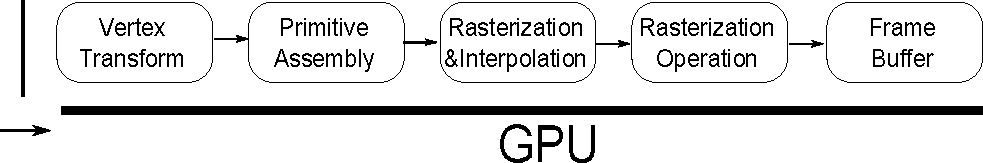
\includegraphics[scale=0.7]{figFixedPipeline.pdf}} 
    \renewcommand{\thefigure}{\thechapter.\arabic{figure}}
    \caption[Fixed-function pipeline]{\emph{Fixed-Function Pipeline}}
    \label{fig:fixed_function_pipeline} 
\end{figure}

% Describe the data type
The modern graphics pipeline is usually designed to take the vertex as the input of data and the vertices are going to be assembled in the pipeline to represent the certain types of geometric primitives (such as triangles) that are going be rendered eventually. The vertices data will be converted into a form that the hardware understands and placed into the vertex cache.  

% Describe the major stages in the pipeline
The major stages in the pipeline will be described in the following text. The first important stage in the pipeline is Transform and Lighting (T\&L). This stage takes the attributes of the vertices, such as the positions, normals, colors and texture coordinates) as input, applies the transformations on each vertices and performs the per-vertex shading calculations according to the light source properties and certain vertex properties. All the output of this stage are per-vertex values.

And the triangle setup stage further creates edge equations that are used to interpolate colors and other per-vertex data across the pixels touched by the triangle in the rendered image. After this stage, it is ready to determine the which pixels are contained in each triangle, this is done by the rasterization stage, at this point, the geometric polygons in the 3D space will be converted to the filled pixels in 2D space, and for each of these pixels, the rasterization process will interpolate per-vertex values neccessary for shading the pixels, including the color, position and texture coordinates that will be shaded (painted) on the pixel.

The next important stage is the shading. As the name implies, the final color of each pixel will be determined in this stage. Many image-based shading techniques and post-processes can be applied here: interpolation of vertex colors, texture mapping, per-pixel lighting calculations and the list goes on and on. 

Following the rasterization stage, the raster operation stage, also known as pixel engines, performs the final raster operation on each pixel. It performs color raster operations that blend the color of overlapping/adjacent objects for transparency and anti-aliasing effects. It also determines the visible objects for a viewpoint and discards the occluded pixels. A pixel becomes occluded when it is blocked by pixels from other objects according to the given new point. 

Finally, the frame buffer interface is responsible for managing the memory reads from and writes to the display frame buffer memory.   

For a couple of decades, each generation of hardware and its corresponding generation of API brought incremental improvements to the various stages of the graphics pipeline, however, developers are always asking for more new features than the build-in function can provide. Therefore, an obvious evolution for the graphics pipeline is the programmable graphics pipeline.   

\paragraph{Programmable Graphics Pipeline}
Programmable graphics pipeline takes a further step by making certain stages into programmable processors. In graphics pipeline, certain stages do a great deal of floating-point arithmetic on completely independent data, in theses stages certain functions will be applied to each element in a set of data (a stream), such as the transformation on the set of vertices positions and pixels shading calculations on the pixel stream. This data independence is one of the key difference between the design assumption for GPU and CPU, this provides a tremendous opportunity to exploit the data parallelism. 

The specific functions executed in the graphics pipeline may vary with rendering algorithms. Such variation became the motivation to make those pipeline stages programmable. There are two particular stages functions have been turned into programmable processors: the vertex shader and pixel shader. 

The vertex shader programs replace the built-in vertex T\&L stage function in the fix-pipeline and runs once on each vertex of the vertex stream the pipeline receives. Typically they perform the essential transformation of the vertex from 3D world space to 2D projection space and per-vertex shading calculations  according to the properties of vertices and light sources. All the properties of a vertex such as positions, colors and texture coordinates can be manipulated in vertex shader by the customized algorithms.   

The pixel shader program is the alternative to the shader stage in the fixed-function pipeline. The essential task of pixel shader program is to compute the color and other attributes of each pixel in the rendered image, lots of image-based algorithms and techniques are implemented in pixel shader programs to achieve some complex per-pixel effects. 

For all the types of shader programs, the program instances can be running in parallel, since the functions are applied on each independent element in a data stream and independent result is produced. This property has motivated the design of the programmable pipeline stages into massively parallel processors.   

The figure ~\ref{fig:ProgrammablePipeline} shows an example of a programmable pipeline that contains a vertex processor and a pixel processor. It is basically a mix of programmable stages and fix-function stages. Between the programmable stages, there are dozens of fixed-function stages that provides much better performance than the programmable stages and benefits much less from programmability. For example, the rasterization which resides between the vertex shader and pixel shader in the pipeline is a completely hardware-implemented function so that the efficiency can maximized. This design of graphics pipeline offers both extreme performance and flexibility to achieve more sophisticated effects. 

% @figure: programmable graphics pipeline
\begin{figure}[htp] 
    \centering 
    \fbox{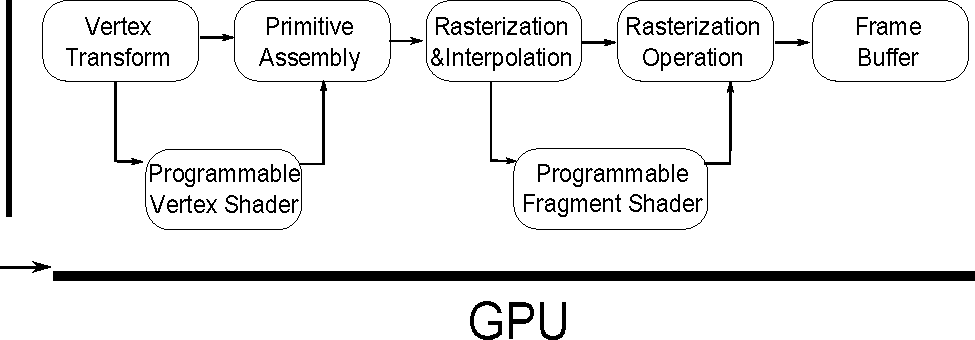
\includegraphics[scale=0.7]{figProgrammablePipeline.pdf}} 
    \renewcommand{\thefigure}{\thechapter.\arabic{figure}}
    \caption[Programmable Graphics Pipeline]{\emph{Programmable Graphics Pipeline}}
    \label{fig:programmable_pipeline} 
\end{figure}

\paragraph{Unified Shaders}
The latest step in the evolution from hardwired pipeline to flexible computational fabric is the introduction of unified shaders, Unified shaders pipeline was first implemented in the ATI Xenos chip for the Xbox 360 gaming console, and the NVIDIA GeoForce 8800 GPU. Instead of separate custom processors of vertex shaders, geometry shaders and pixel shaders, a unified shader architecture provides one large grid of general data-parallel floating-point processors to run all the shader workloads, as illustrated in figure \ref{fig:unified_shaders_pipeline}. This grid of processors can be considered as a pool of unified computational resources, since different applications or even two frames within one application may vary greatly in the demand for various shaders, the array of processors can be allocated dynamically for the demand to achieve a better overall utilization. For example, a video game might begin with a scene with a detail-textured sky without many triangles, this quickly saturates the pixel shaders in a traditional pipeline, while rendering this scene is almost a trivial task. One millisecond later, a scene with highly detailed geometry to draw intricate characters and objects will be rendered, this task will require much more computational power for vertex processing and leave pixel shaders mostly idle. With traditional programmable pipeline, these dramatic changes on in resource demands can vary unpredictably as the players' viewpoint and action change. A unified shader architecture, on the other hand, can allocate a varying percentage of its pool of processor to each shader type. 

% @figure: unified shaders graphics pipeline
\begin{comment}
\begin{figure}[htp]
    \centering 
    \fbox{\includegraphics{.pdf}} 
    \label{fig:unified_shaders_pipeline} 
    \renewcommand{\thefigure}{\thechapter.\arabic{figure}}
    \caption[Unified Shaders Graphics Pipeline]{\emph{Unified Shaders Graphics Pipeline}}
\end{figure}
\end{comment}

\section{General Purpose GPU}
% the motivation
The raw computational power of GPUs growing rapidly beyond everyone's expectation: A single GeForce 8800 chip achieves sustained 330 billion floating-point operations per-second(Gflops) on simple benchmarks. The ever-increasing computational power, programmability, and precision of GPUs has drawn a great deal of interests of performing general-purples computation utilizing GPUs hardware, rather than limiting the application of such a powerful device on image-synthesis. GPGPU stands for General-Purpose computing on graphics on GPU.

% the flexibility

% the limitation of API and new programming language
Although the raw computational power of GPUs has been explosively boosted, accessing the computational resources for general numeric applications is limited by the graphics API. Since the DirectX (before DirectX 10) or OpenGL a programmer had to cast the problem into native graphics operations so that the computation could be launched through DirectX or OpenGL. For example, to pass the data to GPU, the input data has to be stored in texture images, the computation has to be written as a pixel shader and the output has to to be cast as a set of pixels generated from the raster operations.

% not all the applications are suitable for GPGPU
The opportunities always come along with challenges. The specialized architecture of GPU is not well suited to every algorithm. Many applications are inherently serial and are characterized by incoherent and unpredictable memory access. While those applications that may benefit greatly  from the massive parallel architecture shares certain common characteristics: they require significant computational resources and the operate on a large chunk of data which can be mapped well to the GPU's streaming memory subsystem. Porting a judiciously chosen algorithm to the GPU often produces speedups of five to 20 times over optimized CPU codes running on state-of-art CPUs, and speedups of more than 100 times have been reported for some algorithms that map especially well.

%\begin{figure}[htp] 
%    \centering 
%    \fbox{\includegraphics[width=\linewidth]{.pdf}} 
%    \label{fig:GPGPUArch} 
%    \renewcommand{\thefigure}{\thechapter.\arabic{figure}}
%    \caption[]{\emph{}}
%\end{figure}

% CUDA programming concepts
\subsection{GPGPU Programming Concepts}

\subsubsection{Kernels}
Due to the restriction of the programmable shaders graphics pipeline, programmers can be only able to create vertex, geometry and fragment programs that only works on the very limited type of the elemments of the data stream (vertices and fragments). With the generalized type of the elements of the stream data, a generalized version of the programs running on the GPU called \emph{Kernels} is introduced as well. Similar to the programmable shaders, kernels are the functions that are applied to each element in the stream independently performing general computing task.

\subsubsection{Memory Model}



\subsubsection{Thread Hierarchy}


\section{KD-Tree Construction Using GPU}
In Chapter 3, we have defined a fast kd-tree construction algorithm \ref{algo:FindBestPlaneON} that has time complexity of \mycomplexitynlogn. Provided with a powerful modern GPU, it would be fascinating to optimize the algorithm for GPU to fully exploit the fine-grained parallelism of modern GPU architecture. 

%\refs:
% nvidia cuda programming guide

\subsection{Introduction}

In designing a kd-tree algorithm for the GPUs, how to maximally exploit the GPU's streaming architecture to parallelize the kd-tree construction. As discussed in the previous section, the massive parallel architecture of GPU requires \(10^{3}\) to \(10^{4}\) threads for optimal performance \cite{}<++>. The traditional optimized kd-tree construction algorithm adopt DFS (Depth-First Search) scheme to build a kd-tree, while CPU-based parallelized algorithm resort to DFS when the building process reaches a certain level. However, DFS order is not feasible when the algorithm comes to GPU, since the coherency of memory access is critical to GPU. BFS (Breadth-First Order) is an intuitive alternative approach, indeed BFS algorithm is much more suitable to take advantage of the GPU's architecture. Instead of finding split plane for each node greedily, by following BFS order the tree will be built level by level, every node at the same tree level spawns a new thread and the total number of threads doubles from the preceding step. This approach can fully exploit the massive data parallelism of GPU.

Memory management has always been a critical factor that has huge impact on the performance and feasibility of the both CPU and GPU kd-tree constructor. Dynamically allocating memory for kd-tree nodes and their AABBs as the building process goes will hurt the performance greatly making the algorithm unacceptably slow, this is mainly due to the overhead of memory management API on both CPU and GPU. This overhead can be reduced by pre-allocating a chunk of memory that is big enough to hold all the data dynamically created in the kd-tree construction. However, on the other hand, this lead to higher memory requirements as the scene complexity grows and potential memory wastage. More sophisticated memory scheme will be required. The memory management issue will be discussed later in the following chapter.

Another issue is the efficiency of the calculation of the node split costs. The previously described SAH method is important for maintaining the quality of kd-tree. However, precisely evaluating the costs of all the kd-tree nodes is too expensive for real-time applications. Therefore, vary recent approaches sacrificed SAH evaluations picking the median split instead until a certain level reached. Since the as the building process continues, the number of the triangles contained in a voxel of kd-tree node becomes smaller, leading less expensive SAH evaluation iterating over all the triangles. Therefore the number of triangles in an AABB is used as a threshold and it will be specified by the user. 

\subsection{Algorithm Description}
In this section, the GPU-based SAH kd-tree building algorithm will be presented. This algorithm follows the essential scheme as the construction algorithms previous described, it is a greedy, top-down manner as described in the following algorithm. 

\SetAlFnt{\small}
\begin{algorithm}[H]

        \SetKwFunction{buildKDTreeGPU}      {buildKDTreeGPU}
        \SetKwFunction{processLargeNodes}   {processLargeNodes}
        \SetKwFunction{processSmallNodes}   {processSmallNodes}
        \SetKwFunction{outputTreeNodes}     {outputTreeNodes} 

        \myfunc \buildKDTreeGPU{\mytriangles} \newline
        \Begin{
        \tcp{initialization stage}
        \emph{new} treeNodesList 

        \emph{new} workNodesList  
        \emph{new} smallNodesList
        \emph{new} nextNodesList    

        Create rootNode
        workNodesList.add(rootnode)

        \ForEach {\mytriangle\ \(\in\) \mytriangles} \bf in parallel
        {
        Calculate AABB for triangle \mytriangle
        }

        \tcp{process large node}
        \While{workNodesList is not empty} 
        {
        append workNodesList to treeNodesList
        clear nextNodesList
        \processLargeNodes{workNodesList, smallNodesList, nextNodesList}
        Swap nextNodesList and workNodesList
        }

        \tcp{process small node}
        \processSmallNodes{smallNodesList}
        workNodesList \leftarrow\ smallNodesList
        \While{workNodesList is not empty} 
        {
        append workNodesList to treeNodesList
        clear nextNodesList
        \processSmallNodes{workNodesList,nextNodesList}
        Swap nextNodesList and workNodesList
        }

        \tcp{output the kd-tree nodes}
        \outputTreeNodes{treeNodesList}
        }

        \caption{The \mynaive\ algorithm of finding the best SAH split plane}
        \label{algo:BuildKDTreeGPU} 
\end{algorithm}



\SetAlFnt{\small}
\begin{algorithm}[H]
    
    \SetKwFunction{processLargeNodes}       {processLargeNodes}
    
    \myfunc \processLargeNodes{ { {\bf in} workNodesList, {\bf out} smallNodesList, {\bf out} nextNodesList} 
    \Begin {
        \tcp{first step: group triangles into chunks}
        \ForEach{node \mynod\ in workNodesList \bf in parallel}
        {
            Group all triangles in \mynode into fixed size chunks
            Store the chunks in trianglesChunkList
        }

        \tcp{second step: compute per-node AABB}
        \ForEach{chunk \mytrichunk\  in trianglesChunkList \bf in parallel} 
        {
            Calculate the AABB of all triangles in \mytrichunk\ using standard reduction
        }
        Perform segmented reduction on per-chunk reduction result to compute per-node AABB

        \tcp{third step: split large nodes}
        \ForEach{node \mynode\ in workNodesList \bf in parallel}
        {
            \ForEach{side \myaabbside\ of the AABB of node \mynode\ }
            {
                \If{\mynode\ contains empty space larger than a threshold on side \myabbside}
                {
                    Cut off the empty space of \mynode\ on side \myaabbside\ 
                }
            }
            Split node \mynode at spatial median of the longest axis. 
            Two new child nodes are created.
            \ForEach{newly created child node \mynode\ }
            {
                add \mynode to nextNodesList
            }
        }
        
        \tcp{forth step: classify the triangles into child nodes}
        \ForEach{triangles chunk \mytrichunk\ in trianglesChunkList \bf in parallel}
        {
            \mynode \leftarrow the index of the node the chunk \mytrichunk belongs to
            \ForEach{triangle \mytriangle\ in \mytrichunk\ \bf in parallel} 
            {
                \If{\mytriangle\ intersects both child nodes of \mynode\ }
                {
                    \mylefttrilist\  \leftarrow \mytriangle
                    \myrighttrilist\ \leftarrow \mytriangle
                }
                Classify \mylefttrilist\ and \myrighttrilist\ into two child nodes.
                
                \Else {
                    Classify \mytriangle into the child node contains it    
                }
            }
        }

        \tcp{count triangles for child nodes}
        \ForEach{chunk \mytrichunk\ in the trianglesChunkList \bf in parallel}
        {
            \mynode \leftarrow the index of the node the chunk \mytrichunk belongs to
            Count triangles in the child nodes of \mynode.
        }
        
        \tcp{small node filtering}
        \ForEach{child nodes \mynode\ in nextNodesList \bf in parallel}
        {
            \If{\mynode\ is small node}
            {
                Add \mynode\ to smallNodesList
                Delete \mynode from nextNodesList
            }
    }
    \label{algo:ProcessLargeNodes}
\end{algorithm}

\SetAlFnt{\small}
\begin{algorithm}[H]
    \SetKwFunction{ProcessSmallNodes}           {ProcessSmallNodes} 

    \myfunc \ProcessSmallNodes{ {\bf in} workNodesList, {\bf out} nextNodesList }
    }

\end{algorithm}




